\documentclass[journal]{IEEEtran}
\usepackage[caption=false,font=footnotesize]{subfig}
\usepackage{booktabs}
\usepackage{datatool}
\usepackage{diagbox}
\usepackage{listings}
\usepackage{makecell}
\usepackage{tikz}
\usetikzlibrary{positioning}
\usetikzlibrary{trees}
\usetikzlibrary{fit}
\usetikzlibrary{backgrounds}
\usepackage[hyphens]{url}
\usepackage{hyperref}

\lstdefinestyle{lststyle}{
	aboveskip=10pt,
	belowskip=10pt,
	frame=single,
	basicstyle=\tt\scriptsize,
	commentstyle=\color{gray}}

\begin{document}
\DTLloaddb{keys_values}{results/keys-values.csv}

\title{Reproducible Builds for\\ Computational Research Papers}

\author{Paschalis~Bizopoulos and Dimitris~Bizopoulos
\thanks{P. Bizopoulos and D. Bizopoulos are Independent Researchers, Thessaloniki, Greece e-mail: pbizopoulos@protonmail.com, dimitrisbizopoulos@gmail.com}}

\maketitle

\begin{abstract}
	Previous works in research reproducibility provided frameworks for writing reproducible research papers, however without considering the cost of extra work that needs to be done by the author to make the paper reproducible and by the reviewer to verify the paper's reproducibility.
	We propose a simple template for writing computational research papers in \LaTeX\ that are easily verifiable in terms of their reproducibility.
	The template contains a Makefile that allows the author/reviewer to execute the code that reproduces the figures, tables and variables (results) of the paper, which are then used during the \LaTeX\ compilation, to produce a pdf.
	The previous procedure is completed twice and the paper is verified as reproducible, if and only if the pdf files are identical.
	The two builds are needed to enable comparison between different builds of the same source code such that any non-deterministic stochasticity would produce different pdf files, thus making the paper non-reproducible.
	The reproducibility of a paper can be verified either locally on the machine of the reviewer or remotely using Virtual Machines (VMs) in the cloud.
	We release an open source template of \textit{reproducible builds} (RBs) and use it to write and verify the reproducibility of this paper.
\end{abstract}

\section{Introduction}
A research paper is considered reproducible when any reviewer is able to reproduce its results, given the data and experimental procedure.
More specifically, computational research reproducibility requires the presence of source code that produces or fetches data from external sources which then transforms into the figures, tables and variables of the paper.
Open sourcing the code and the raw data of a computational research paper increases the confidence in its reproducibility but it is not enough to verify it.
Using a template both for writing and verifying computational research papers will push the direction towards creating reproducible research, thus tackling the `reproducibility crisis' problem.

We propose a template for writing computational research papers with \LaTeX\ and verifying  its reproducibility using the concept of \textit{reproducible builds} (RBs) in a local or remote computational environment.
We provide an open source implementation of the template\footnote{\url{https://github.com/pbizopoulos/cookiecutter-reproducible-builds-for-computational-research-papers}}, which we use to write this paper\footnote{\url{https://arxiv.org/abs/2005.12660}} and verify its reproducibility\footnote{\url{https://github.com/pbizopoulos/reproducible-builds-for-computational-research-papers}}.
We use Python~\cite{van2007python} for producing the results, however other scientific-oriented programming languages can be used.

For the rest of the paper we will refer to:
\begin{itemize}
	\item \textit{paper} as a computational research paper,
	\item \textit{results} as the figures, tables and variables that are shown in the \textit{paper},
	\item \textit{\LaTeX\ code} as the files containing the main text (\textit{*.tex}) and bibliography (\textit{*.bib}) of the \textit{paper},
	\item \textit{results code} as the files containing the scientific-oriented programming language code (\textit{*.py}) that produces the \textit{results},
	\item \textit{code} as both the \textit{\LaTeX\ code} and \textit{results code},
	\item \textit{author} as the author(s) of the \textit{paper} and
	\item \textit{reviewer} as the reviewer(s) of the \textit{paper} or anyone interested in verifying the \textit{paper} (author(s), journal editors, other researchers).
\end{itemize}

\section{Reproducible Builds Template}

\begin{figure}[!t]
	\centering
	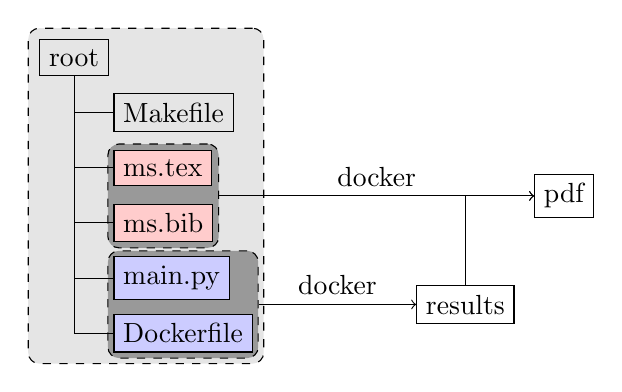
\begin{tikzpicture}[%
			grow via three points={one child at (0.5,-0.7) and two children at (0.5,-0.7) and (0.5,-1.4)},
			edge from parent path={(\tikzparentnode.south) |- (\tikzchildnode.west)}]
			\node[draw](root){root}
			child{node[draw, anchor=west](makefile){Makefile}}
			child{node[draw, anchor=west, fill=red!20](tex){ms.tex}}
			child{node[draw, anchor=west, fill=red!20](bib){ms.bib}}
			child{node[draw, anchor=west, fill=blue!20](py){main.py}}
			child{node[draw, anchor=west, fill=blue!20](dockerfile){Dockerfile}};
			\begin{scope}[on background layer]
				\node[draw, rounded corners, dashed, fill=gray!20, inner sep=4pt, fit=(root) (dockerfile)]{};
				\node[draw, rounded corners, dashed, fill=gray!80, inner sep=2pt, fit=(py) (dockerfile)](code){};
				\node[draw, rounded corners, dashed, fill=gray!80, inner sep=2pt, fit=(tex) (bib)](paper){};
			\end{scope}
			\node[draw, right=2cm of code, fill=white] (results) {results};
			\path[draw, ->] (code) -- node[above]{docker} (results);
			\node[draw, right=4cm of paper, fill=white] (pdf) {pdf};
			\path[draw, ->] (results) |- (pdf);
			\path[draw, ->] (paper) -- node[above]{docker} (pdf);
	\end{tikzpicture}
	\caption{The RBs template file hierarchy is depicted in the light gray background and the arrows denote the data flow towards generating the pdf.
	Blue indicates a \textit{results code} file, red a \textit{\LaTeX\ code} file and within the dark gray background, files that are used for a subsequent step.}
	\label{fig:filehierarchyworkflow}
\end{figure}

The proposed template can be used for writing \textit{papers} with \LaTeX~\cite{lamport1994latex} and the \textit{results code} that can be executed within a Docker container.
\LaTeX\ is a typesetting system for publishing high quality research papers, and Docker~\cite{merkel2014docker} is a container system that allows portable execution of a codebase between different operating systems/environments and has shown great promise in reproducible research~\cite{boettiger2015introduction}.

A specific file hierarchy is shown in Fig.~\ref{fig:filehierarchyworkflow} however this is optional, as the template only needs to know the directories of the main files of the \LaTeX\ and \textit{results code} during its creation.
The Makefile and Dockerfile are automatically generated by the template after user prompts.
For more complicated setups the Dockerfile can be provided by the \textit{author} or generated by tools such as repo2docker~\cite{forde2018reproducible}.

The template fits in research writing and reproducibility verification in the following way:
\begin{enumerate}
	\item the \textit{author} edits the \textit{code} in the local repository,
	\item the \textit{author} may execute \textit{make} during development and experimentation,
	\item the \textit{author} may verify the reproducibility of the \textit{paper} locally by executing \textit{make test} (or remotely by commiting the code change with a message which contains \textit{\{make test\}}) which triggers the following:
		\begin{enumerate}
			\item the \textit{results code} is executed,
			\item the \textit{results} along with the \textit{\LaTeX\ code} are used to compile a pdf file,
			\item the previous is executed twice,
			\item the \textit{paper} is verifed as reproducible if and only if the pdf files are identical.
		\end{enumerate}
	\item the \textit{reviewer} may verify the reproducibility of the paper locally (by cloning the repo and executing \textit{make test}) or remotely (by inspecting the result of \textit{\{make test\}}).
\end{enumerate}

The reason that two local/remote compilations are needed is to enable comparison between different builds of the same source code and any non-deterministic stochasticity (such as not applying a specific seed to random generators) would produce different pdfs, thus making the \textit{paper} non-reproducible.
Moreover Docker usage in RBs provides portability of the environment of the research while third-party VMs are used when the verification needs to be shared (in contrast with verifying locally, thus having low credibility in reporting reproducibility).

Additional constraints could be imposed in the VMs such as disallowing image files in the \textit{code} and monitoring the network connections of the \textit{code} to help the \textit{reviewer} check whether the \textit{results} are generated from the \textit{code} and are not fetched from an external source.

Potential uses of the RBs template include:
\begin{itemize}
	\item preprint server (e.g.\ arXiv) \textit{paper} reproducibility verification and
	\item regression testing and debugging, to ensure that changes to \textit{code} do not alter the results.
\end{itemize}

\subsection{Technical implementation}
Executing RBs can be done using the following:
\begin{lstlisting}[language=Bash, style=lststyle, caption={Makefile call syntax from the shell.}, captionpos=b]
SYNTAX
make [OPTION] [ARGS=--full]

OPTIONS
ms.pdf - Generate pdf.
test   - Test whether the paper has a reproducible build.
clean  - Remove cache, results directories and tex aux files.
help   - Show help.

\end{lstlisting}

\begin{table}[]
	\centering
	\caption{Makefile usage table.}
	\label{table:usagetable}
	\begin{tabular}{l|l|l}
		\toprule
		\diagbox{\textbf{OPTION}}{\textbf{ARGS}} & \textbf{(empty)}              & \textbf{-{}-full}                    \\
		\midrule
		\textbf{(ms.pdf or empty)}          & debug/development    & release paper             \\
		\midrule
		\textbf{test}                       & test reproducibility & test reproducibility full \\
		\bottomrule
	\end{tabular}
\end{table}

Regarding research that is computational costly, the template allows the execution and reproducibility verification of a computationally lighter version of the \textit{paper} by default.
This also helps in faster iterations during research writing and experimentation.
An example of computationally lighter versions in the field of neural networks is setting the number of epochs and number of training samples to a low value.
The execution of the full experiment is done by providing an additional argument.

The RB template takes advantage of the automatic generation of intermediate files of the `make' program.
The \textit{author} only needs to edit (or use the `touch' UNIX utility to update the modification time) a file from \textit{results code} or \textit{\LaTeX\ code} and the corresponding compilation is automatically triggered with `make'.

In this implementation of RBs the remote reproducibility verification is done using Github Actions, the builder VM uses the latest version of Ubuntu and pulls a docker image for building \LaTeX\ from the Github Container Registry.

\section{Example Use Case of RBs}
This sections provides a use case of RBs and also serves as a manual for creating reproducible \textit{papers} written in \LaTeX\ with Python as the \textit{results code} programming language.
For demonstration purposes we train and test a VGG11 neural network~\cite{simonyan2014very} with batch normalization in PyTorch~\cite{paszke2019pytorch}, on the following datasets:
\begin{itemize}
	\item MNIST~\cite{lecun2010mnist},
	\item FashionMNIST~\cite{xiao2017fashion},
	\item KMNIST~\cite{clanuwat2018deep},
	\item QMNIST~\cite{yadav2019cold},
	\item EMNIST~\cite{cohen2017emnist},
	\item CIFAR10~\cite{krizhevsky2009learning},
	\item CIFAR100~\cite{krizhevsky2009learning} and
	\item SVHN~\cite{netzer2011reading}.
\end{itemize}

We split to train, validation and test datasets and compare the use of ReLU and SELU activation functions in a VGG11 model.
The images from the MNIST variants are resized to $32\times 32$ to comply with the dimensions of VGG11.
Regarding \LaTeX\ a common culprit against reproducibility is the time-date metadata embedded in the pdf output.
These can be disabled using the following commands into the \textit{\LaTeX\ code} or as extra arguments during \LaTeX\ compilation (as done in the RB Makefile):
\begin{lstlisting}[language=TeX, style=lststyle, caption={\LaTeX\ pdf reproducibility commands.}, captionpos=b]
\pdfinfoomitdate=1
\pdfsuppressptexinfo=-1
\pdftrailerid{}
\end{lstlisting}

A useful \LaTeX\ package for automatically embedding variables from \textit{results} in \textit{\LaTeX\ code} is \textit{datatool} with the following example use:
\begin{lstlisting}[language=TeX, style=lststyle, caption={\LaTeX\ datatool example of loading a file that contains pairs of keys and values (keys\_values.csv) generated by a \textit{results code} and getting the value of a key named lr.}, captionpos=b]
\DTLloaddb{keys_values}{keys_values.csv}
\DTLfetch{keys_values}{key}{lr}{value}
\end{lstlisting}

For example the values of the following variables are not referred in the main \textit{.tex} file but they are read by an intermediate \textit{.tex} file created by the \textit{results code}:
\begin{itemize}
	\item the number of epochs is $\DTLfetch{keys_values}{key}{num_epochs}{value}$,
	\item the batch size is $\DTLfetch{keys_values}{key}{batch_size}{value}$ and
	\item the learning rate for SGD is $\DTLfetch{keys_values}{key}{lr}{value}$.
\end{itemize}

Regarding the \textit{results code} for Python, random seeds need to be set to a specific value such as:
\begin{lstlisting}[language=python, style=lststyle, caption={Python reproducibility commands for some popular libraries.}, captionpos=b]
# for build-in random module
random.seed(0)
# for numpy
np.random.seed(0)
# for tensorflow
tf.random.set_seed(0)
# for pytorch
torch.backends.cudnn.benchmark = False
torch.backends.cudnn.deterministic = True
torch.cuda.manual_seed_all(0)
torch.manual_seed(0)
\end{lstlisting}

Using the random seeds and \textit{datatool} we could have deterministic stochasticity that reproduces figures, tables and variables.
For example Fig.~\ref{fig:image} depicts the train and validation loss for all datasets.
\begin{figure}[!t]
	\subfloat{\includegraphics[width=0.25\textwidth]{results/MNIST-loss}}
	\subfloat{\includegraphics[width=0.25\textwidth]{results/FashionMNIST-loss}}
	\caption{Train and validation losses for MNIST and FashionMNIST.}
	\label{fig:image}
\end{figure}

Another useful function for Python is \textit{pandas.DataFrame.to\_latex} which automatically converts a dataframe table to a \LaTeX\ table (as shown in Table~\ref{table:table}).

\begin{lstlisting}[language=python, style=lststyle, caption={Convert Pandas DataFrame to \LaTeX\ table.}, captionpos=b]
num_columns = 11
table = np.random.random((7, num_columns))
df = pd.DataFrame(table)
df.to_latex('metrics.tex', float_format="%.2f")
\end{lstlisting}

\begin{table}[h]
	\centering
	\caption{Table example created from results code.}
	\label{table:table}
	\setlength\tabcolsep{4.2pt}
	\scalebox{0.72}{\input{results/metrics.tex}}
\end{table}

\section{Discussion}
RBs are based on plain text files and are independent of any specific version control and docker registry providor thus preventing `vendor lock-in' situations.
Previous works in this area such as Hurlin et al.~\cite{hurlin2019reproducibility} propose an `external certification agency' for economic studies.
RBs provide a simple solution for writing and verifying the reproducibility of a `\textit{paper} as a whole', without having to trust a third-party.
Anyone can clone a repository written with RBs and locally verify its reproducibility, in case third party VMs cannot be trusted.
Similar to RBs is ReDoc~\cite{schwab2000making} which however focuses on separate result file reproducibility and requires the author to write each rule in the Makefile for each result file.
RBs on the other hand provides a Makefile that is automatically generated by the template.

\section{Conclusion}
Automating research reproducibility verification is becoming more important due to the increasing research output that has been observed in the last few years.
Few works were done on this area, mostly proposing trust on an external third party.
RBs help in writing and verifying reproducible research using the tools that most of the researchers already use (\LaTeX, Docker).

\bibliographystyle{IEEEtran}
\bibliography{ms}

\end{document}
